\documentclass[9pt,mathserif]{beamer}

%% \usepackage{pgfpages}
%% %\setbeamertemplate{note page}[plain]
%% %\setbeameroption{show notes on second screen=bottom}

\usepackage[spanish, es-noshorthands]{babel} 
\usepackage[utf8]{inputenc}

\usepackage{textpos} %textblock
%% \usepackage{tikz,pgfplots}
%% %\setbeamertemplate{navigation symbols}{}

%% %%%%\usecolortheme{rose}
%% %\usecolortheme{seahorse}
%% %\usetheme{Copenhagen}
%% %\usetheme{Warsaw}
\usetheme[width=3\baselineskip]{Berkeley}
\usecolortheme{spruce}   % color verde lindo
\definecolor{forestgreen}{rgb}{0.0, 0.27, 0.13}
\setbeamercolor{itemize item}{fg=forestgreen}
\setbeamercolor{block title}{bg=forestgreen!12,fg=forestgreen}
%% \usecolortheme{beaver}



\usepackage{subfigure}
\setbeamertemplate{caption}{\raggedright\insertcaption\par}
\setbeamerfont{caption}{size=\scriptsize}
\setlength{\abovecaptionskip}{5pt plus 3pt minus 2pt}

% TITLE PAGE ----------------------------------------------------------------------------------
%\logo{
\includegraphics[width=0.75cm,height=0.75cm]{figuras/ib.png}}

\title[]{MODELADO COMPUTACIONAL DEL COMPORTAMIENTO HIDRODINÁMICO DE ELEMENTOS COMBUSTIBLES NUCLEARES}
\author[]{\large{Julia Martorana, Exequiel Fogliatto, Federico Teruel, Enzo Dari y Mariano Cantero}}
\institute{\normalsize{Departamento de Mecánica Computacional \\ Centro Atómico Bariloche \\  Comisión Nacional de Energía Atómica \\  Instituto Balseiro - Universidad Nacional de Cuyo}}
\date{}
% -----------------------------------------------------------------------------------------------

\begin{document}
\renewcommand{\tablename}{}                         % Reemplaza la palabra Cuadros, por 'nada' 
\renewcommand{\figurename}{}                        % Reemplaza la palabra Cuadros, por 'nada'

\begingroup
\makeatletter
\setlength{\hoffset}{-.5\beamer@sidebarwidth}
\makeatother
\begin{frame}[plain]
  \titlepage
  \begin{textblock}{5}(-0.5,-0.25)
    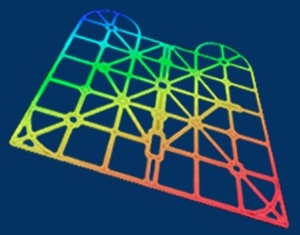
\includegraphics[width=1.15cm]{figuras/ENIEF2017.png}
  \end{textblock}
  \begin{textblock}{5}(12.25,-0.5)
    
\includegraphics[width=1.15cm]{figuras/CNEA.jpg}
  \end{textblock}
  \centering
  \normalsize{XXIII Congreso sobre Métodos Numéricos y sus Aplicaciones} \\
\end{frame}
\endgroup

% -----------------------------------------------------------------------------------------------
% INDICE 
%% \frame[plain]{
%%   \frametitle{Contenidos}
%%   %	\begin{minipage}{\textwidth}
%%    \tableofcontents 
%%   %\end{minipage}
%% }

%% % -----------------------------------------------------------------------------------------------
 \section{Introducción}

\frame{
  \frametitle{Introducción}
    \begin{figure}[!htb]
    \center
    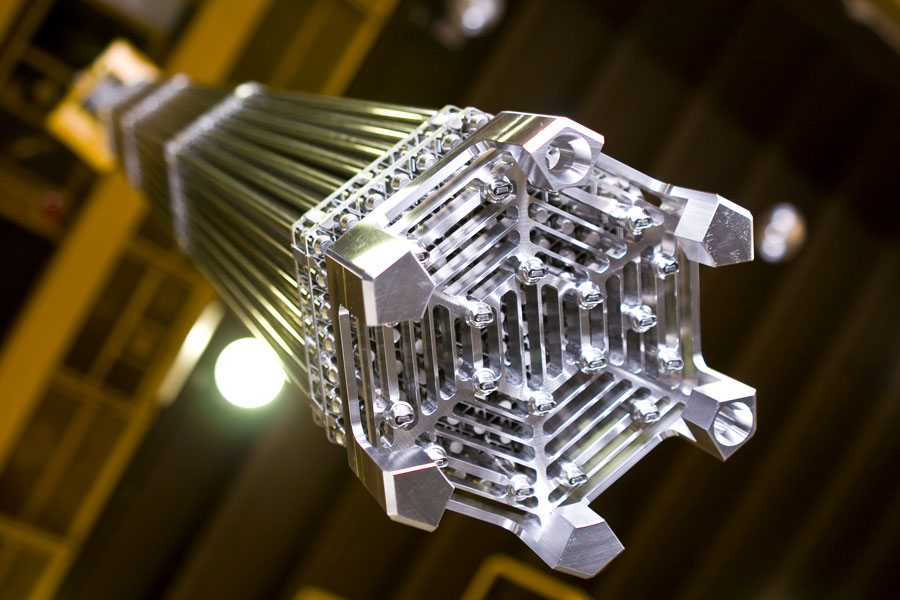
\includegraphics[width=6cm]{figsCAREM/CAREMfromCNEAfuelelement.jpg}
    \caption{Elemento combustible CAREM 25.}
    \end{figure}
    
  - Elementos combustibles\\
  - Características del flujo\\
  - flujo critico de calor, Por qué estudiar \\
  - Objetivo del trabajo en gral y en particular.

}
\section{Herramientas}
\frame{
  \frametitle{Herramientas}

  %\begin{minipage}{0.75\textwidth}
    \begin{block}{SALOME}
      Programa libre que incorpora módulos para generación de modelos CAD y motores de mallado en 3 dimensiones.
      \begin{itemize}
      \item Representación geométrica detallada de los EC.
        \end{itemize}
    \end{block}
    %\end{minipage}
    \vspace{1cm}
  
   %\begin{minipage}{0.75\textwidth}
    \begin{block}{OpenFOAM}
      Conjunto de bibliotecas de C++, destinadas a crear aplicaciones que involucren la resolución de EDP.
      \begin{itemize}
      \item Generación de mallas hexahédricas.
      \item Resolución de ecuaciones RANS mediante FVM.
      \end{itemize}
    \end{block}
    %\end{minipage}

    \note{-SnappyHexMesh es una utilidad de OpenFOAM que permite generar mallas hexahédricas para geometrías arbitrarias. Su desempeño es muy bueno.}

}
 \section{Geometría}
\frame{
  \frametitle{Geometría}
  \framesubtitle{Elemento combustible símil ATUCHA II}


  \begin{columns}
      \hspace{-1cm}
    \column{0.65\textwidth}
    \begin{minipage}[c][0.4\textheight][c]{\linewidth}
     \begin{figure}
       %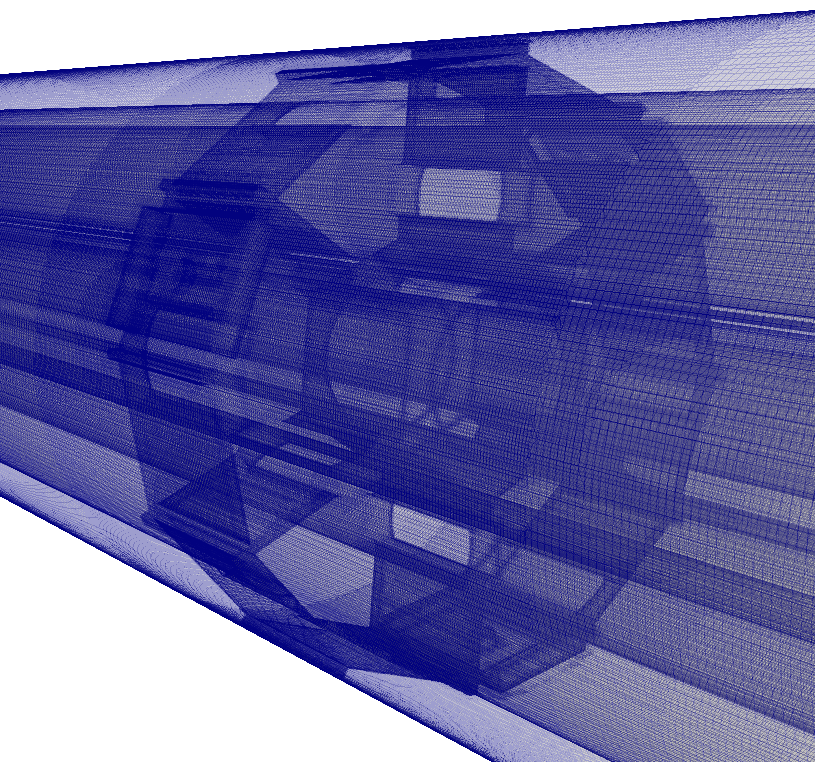
\includegraphics[width=0.55\linewidth]{figsATUCHA/atucha_mesh1a.png}
     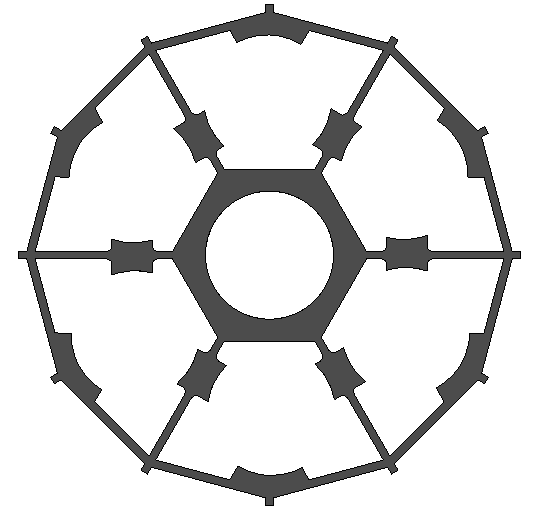
\includegraphics[width=0.525\linewidth]{figsATUCHA/2.png} \vspace{-3mm}
      \caption{Sección transversal del separador}
    \end{figure}
    \end{minipage}

    \vspace{0.5cm}
    \begin{minipage}[c][0.4\textheight][c]{\linewidth}
      \begin{figure}
        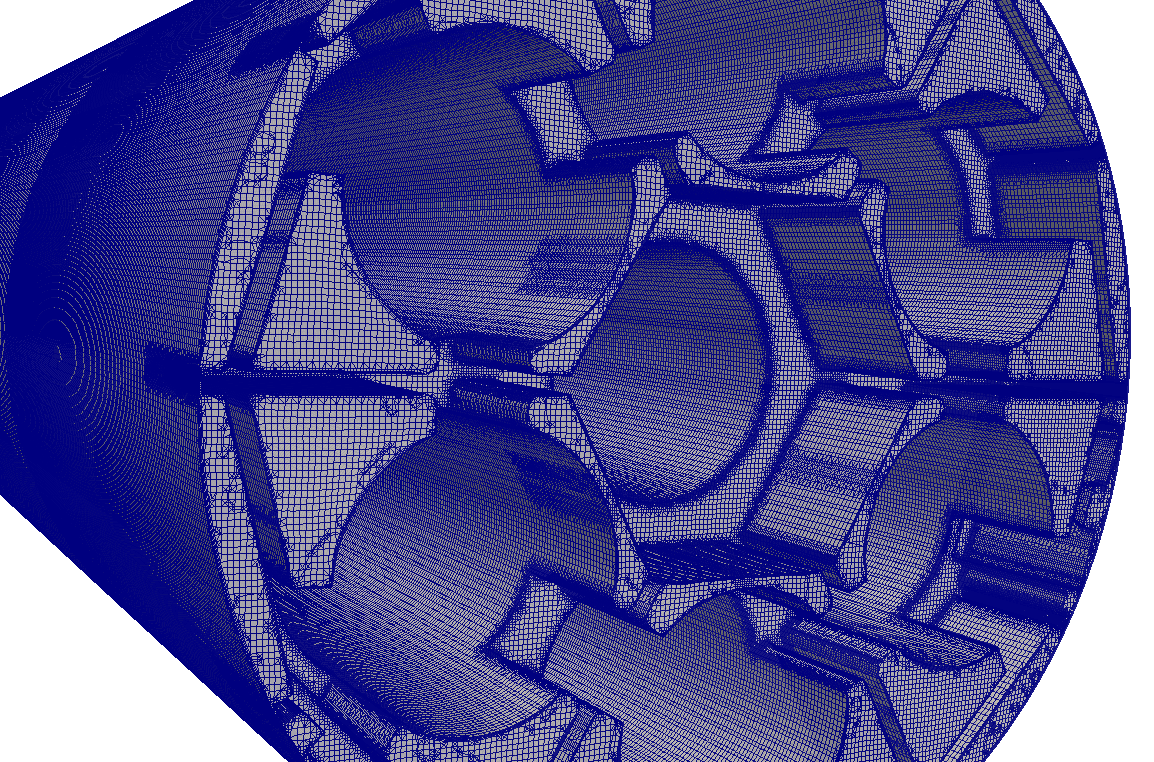
\includegraphics[width=0.65\linewidth]{figsATUCHA/atucha_mesh2a.png} \vspace{-3mm}
        \caption{Corte en el centro del separador.}
      \end{figure}
    \end{minipage}
    
    \column{0.5\textwidth}
    \begin{minipage}[c][0.4\textheight][c]{\linewidth}
      \begin{itemize}
      \item Símil CNAII 7 vainas.
      \item Malla de 14M de celdas.
      \item 4 capas adicionales en bordes.
      \end{itemize}
    \end{minipage}
    
    \begin{minipage}[c][0.5\textheight][c]{\linewidth}
      \begin{figure}
        \hspace{-1.5cm}   
        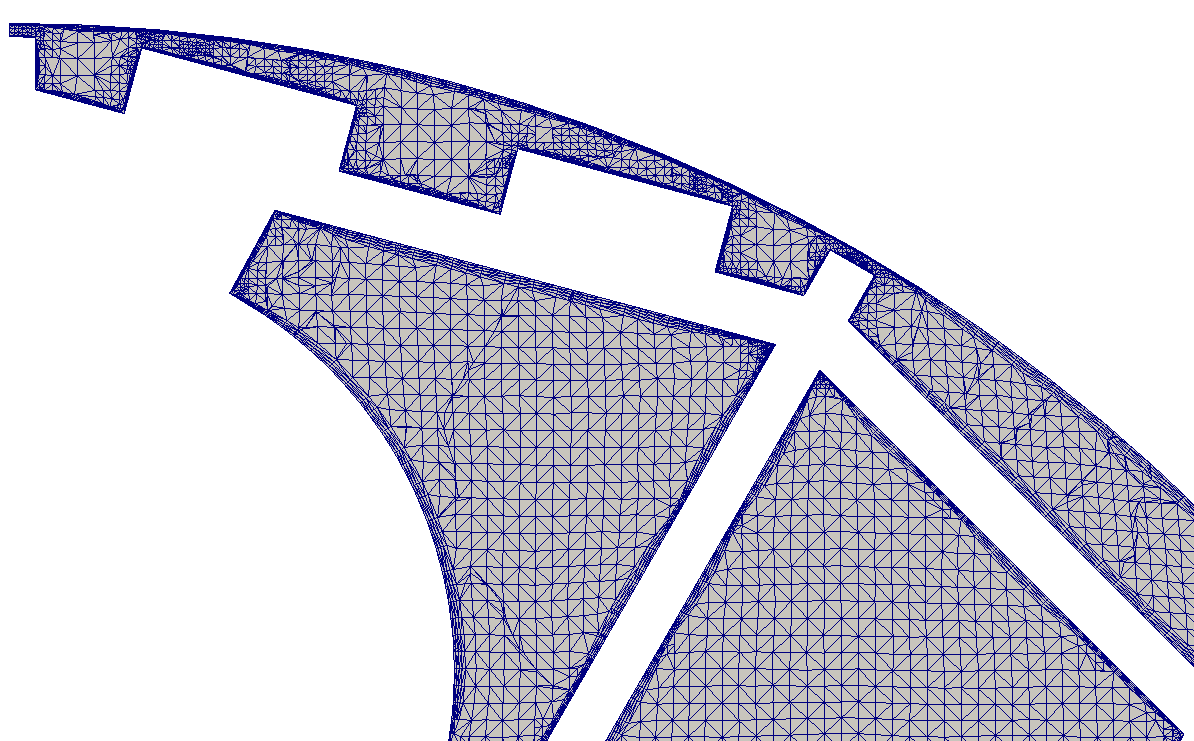
\includegraphics[width=0.95\linewidth]{figsATUCHA/atucha_mesh3a.png} \vspace{-3mm}
        \caption{Detalle de capas adicionales.}
        \end{figure}
    \end{minipage}
  \end{columns}
}

\frame{
  \frametitle{Geometría}
  \framesubtitle{Elemento combustible símil CAREM}
  
%  \vspace{-0.25cm}
  \begin{columns}
    \column{0.65\textwidth}
    \begin{minipage}[c][0.4\textheight][c]{\linewidth}
     \begin{figure}
        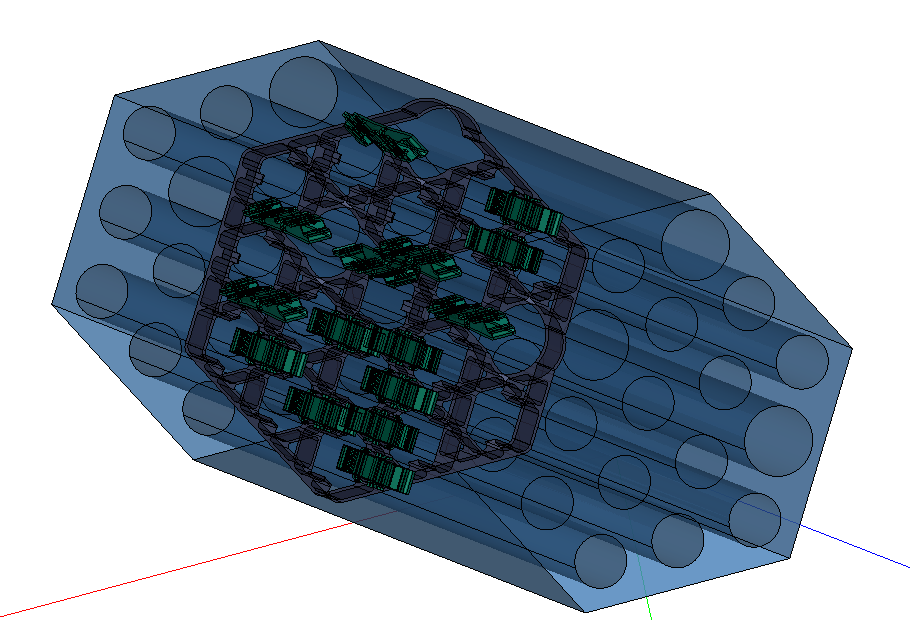
\includegraphics[width=0.85\linewidth]{figsCAREM/CAREM3.png} \vspace{-3mm}
        \caption{Geometría completa.}
    \end{figure}
    \end{minipage}

    %\vspace{0.5cm}
    \begin{minipage}[c][0.4\textheight][c]{\linewidth}

      \begin{itemize}
      \item Símil CAREM de 16 vainas y 3 tubos de control.
      \item Malla de 53M de celdas.
      \item 4 capas adicionales en bordes.
      \end{itemize}
      
    \end{minipage}
    
    \column{0.45\textwidth}
    \begin{minipage}[c][0.4\textheight][c]{\linewidth}
      \begin{figure}
     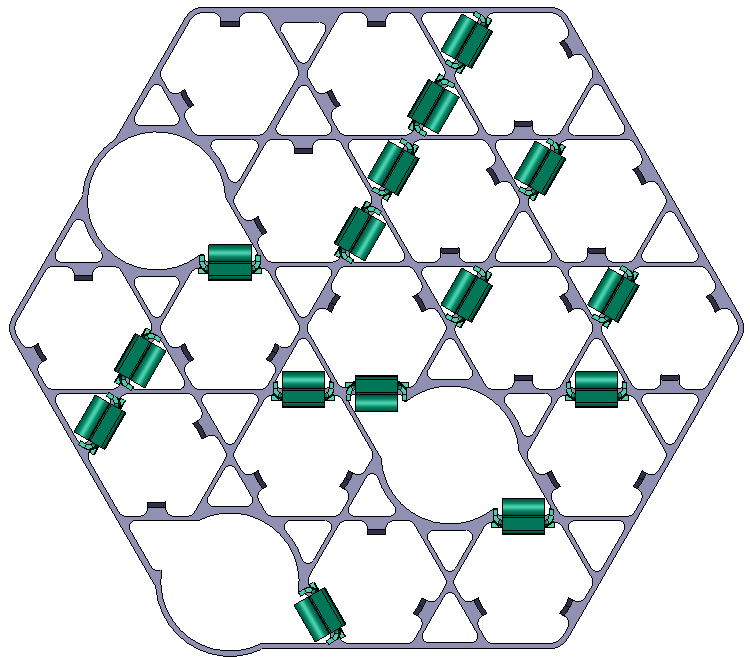
\includegraphics[width=0.8\linewidth]{figsCAREM/CAREM1.png} \vspace{-3mm}
      \caption{Vista de separador y resortes.}
      \end{figure}
    \end{minipage}
    
    \begin{minipage}[c][0.5\textheight][c]{\linewidth}
      \begin{figure}
        %\hspace{-1.5cm}   
        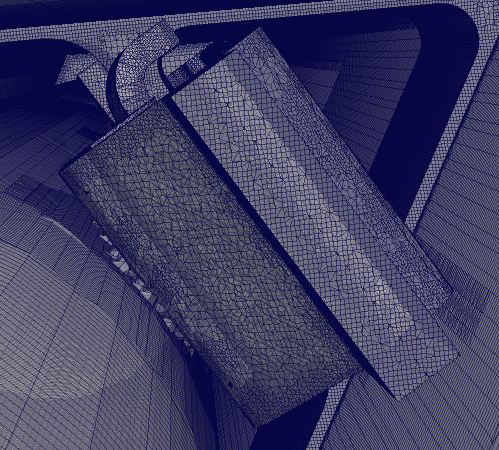
\includegraphics[width=0.75\linewidth]{figsCAREM/mesh_detalle3.png} \vspace{-3mm}
        \caption{Detalle de malla en resorte.}
        \end{figure}
    \end{minipage}
  \end{columns}
 
}

% ===========================================================================================================
\section{Resultados}
\subsection{Modelos de turbulencia}
\frame{
  \frametitle{Modelos de turbulencia}

    \begin{minipage}[c]{0.6\linewidth}
      \begin{itemize}
      \item Geometría: canal circular con 7 vainas.
      \item Análisis de modelos de turbulencia:
      \end{itemize}
    \end{minipage}
    \begin{minipage}[c]{0.3\linewidth}
      \begin{figure}
        \center
      
\includegraphics[width=0.65\linewidth]{figsGEOM/geom_mod_turb.png} \vspace{-3mm}
      \caption{Sección transversal del canal analizado.}
    \end{figure}
    \end{minipage}
    
   \begin{table}[ht]
%      \setlength{\tabcolsep}{10pt}
        \centering
        \begin{tabular}{c c c c }
            \hline
            \bf Modelo & \bf Malla & \bf V. Layer  &  \bf Pendiente \\
            \hline
            $k$ - $\omega$     & 1 / 0.25 & 0.25/10  &  4.364\\
            $k$ - $\omega$ SST & 1 / 0.25 & 0.25/10  &  4.831\\
            Spallart Almaras & 0.125 / 0.125 & 0.25/10  &  4.866\\
            \hline
        \end{tabular}
        \caption{Modelos de turbulencia estudiados.}
    \end{table}    

}

\subsection{EC ATUCHA}
\frame{
  \frametitle{Elemento combustible símil ATUCHA}
  \framesubtitle{Pérdida de carga}
  \begin{figure}[!htb]
    \center
    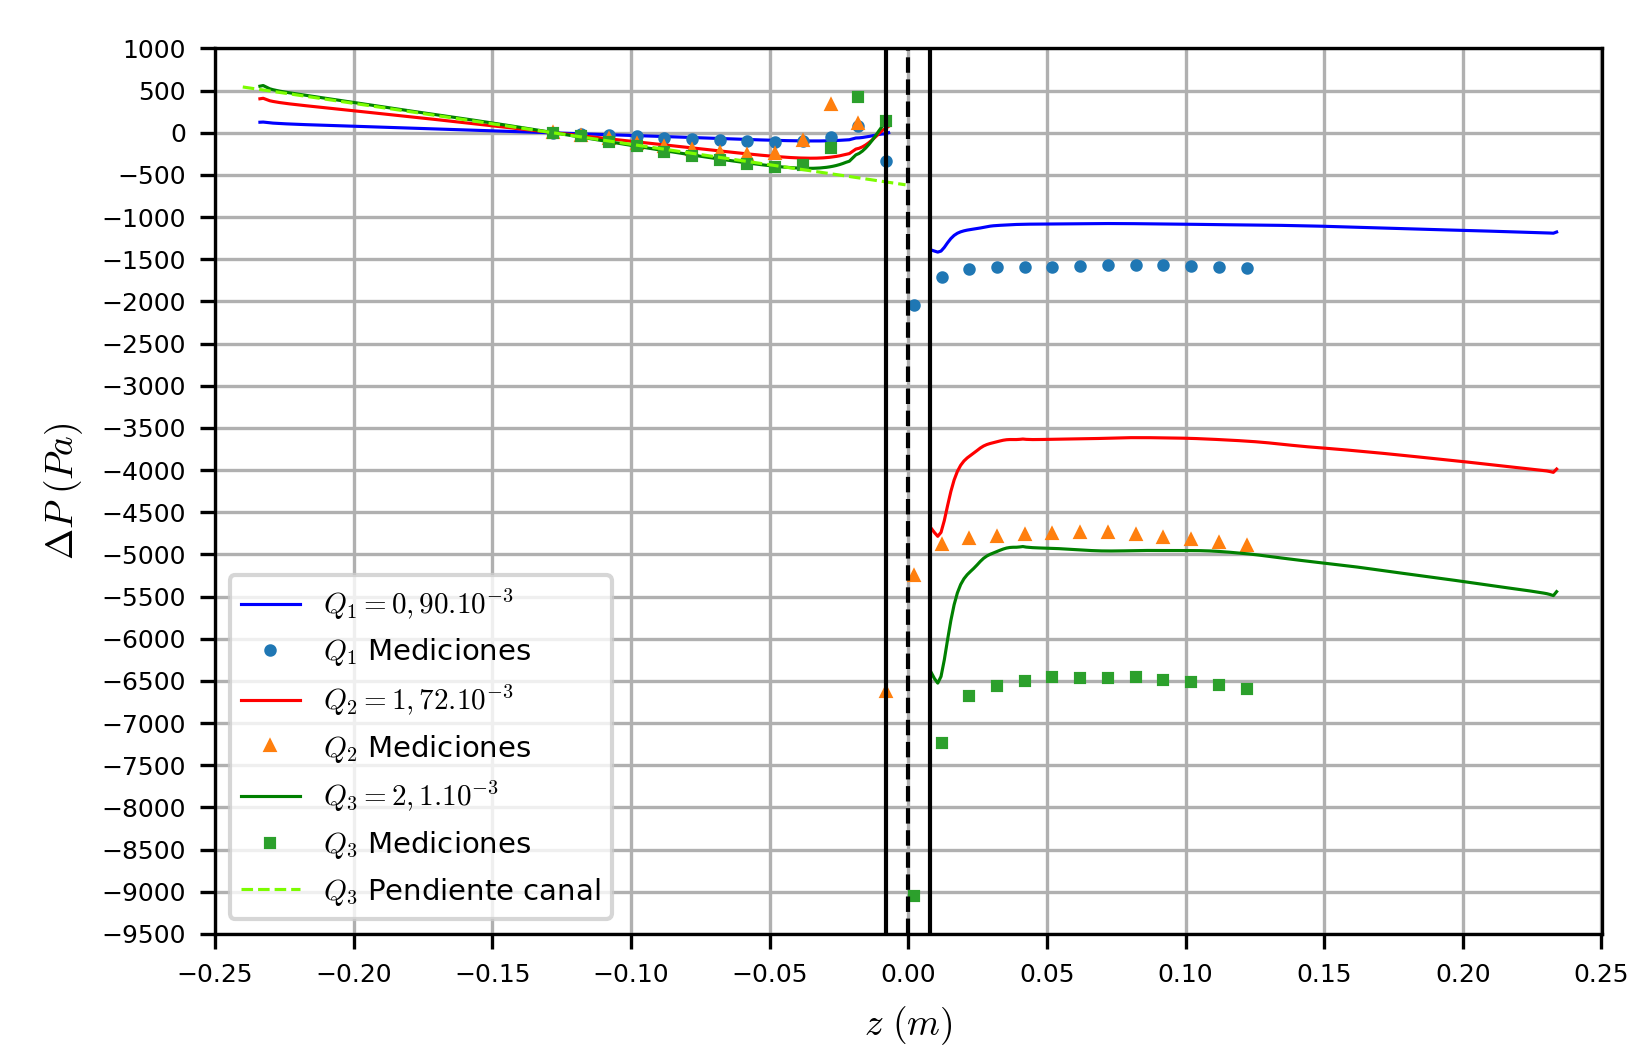
\includegraphics[width=10cm]{figsATUCHA/US_DS.png}
  \end{figure}
}

\frame{
  \frametitle{Elemento combustible símil ATUCHA}
  \framesubtitle{Pérdida de carga}
  \begin{figure}[!htb]
    \center
    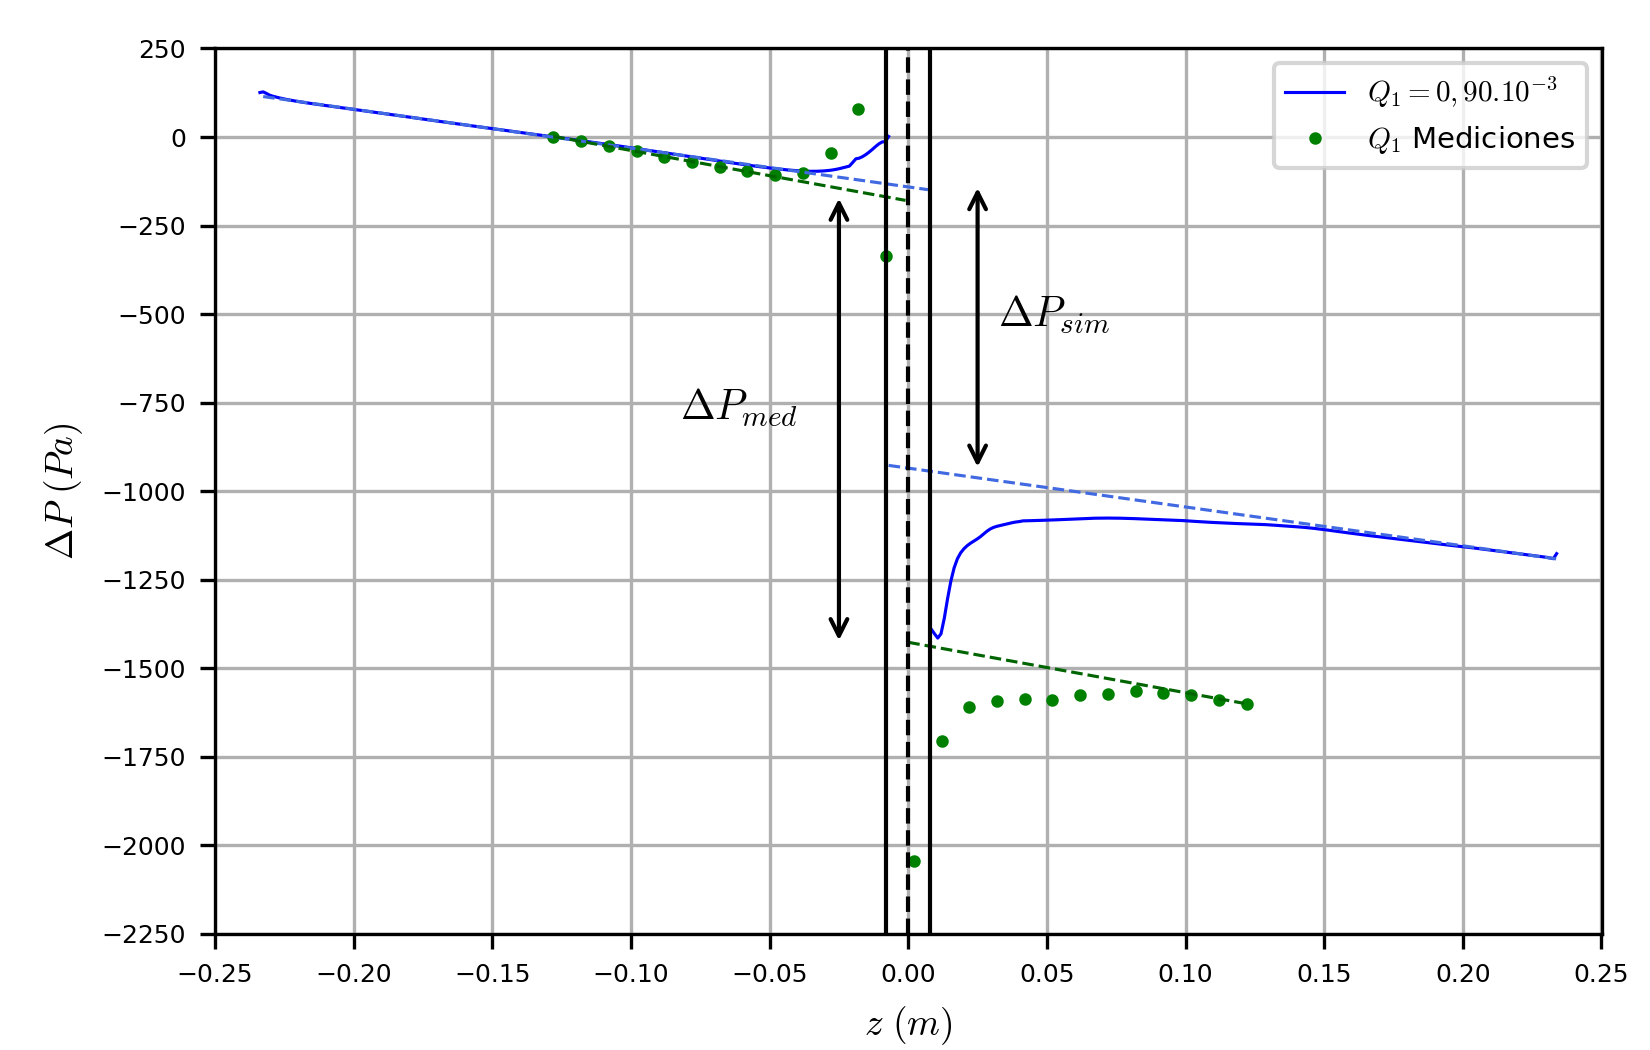
\includegraphics[width=8cm]{figsATUCHA/US_DS_fit_Q1.png}
  \end{figure}

  \begin{table}[ht]
        \centering
        \begin{tabular}{c | c | c | c }
            \bf Caudal $(m^3/s)$  & \bf $\Delta P_{sim}$  & \bf $\Delta P_{med}$ & \bf Diferencia (\%)  \\
            \hline
            \hline
            $Q_1=0.90 10^{-3}$ & 794.15  & 1246.43 & 36.3 \\
            $Q_2=1.72 10^{-3}$ & 2716.69 & 3910.64 & 30.5\\
            $Q_3=2.01 10^{-3}$ & 3640.50 & 5220.35 & 30.3\\
        \end{tabular}
        \caption{Valores de pérdida de carga local.}
        \label{tab:DP}
  \end{table}
  
}
\frame{
  \frametitle{Elemento combustible símil ATUCHA}
  \framesubtitle{Distribución de velocidad principal}
  \begin{figure}[ht]
        \centering
        %\begin{subfigure}[t]{0.45\textwidth}
            \centering
            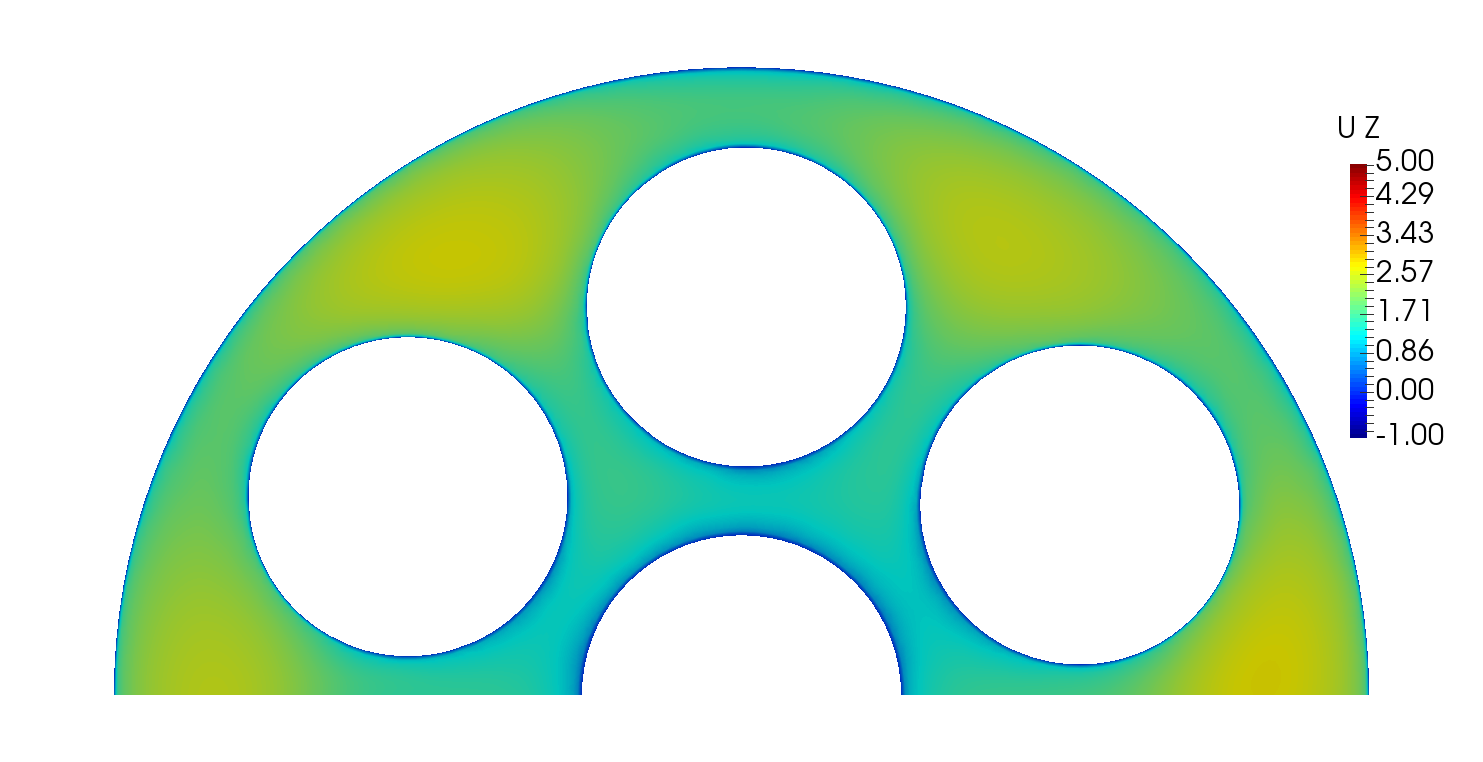
\includegraphics[width=0.45\textwidth]{figsATUCHA/vel/U_0015US.png}
            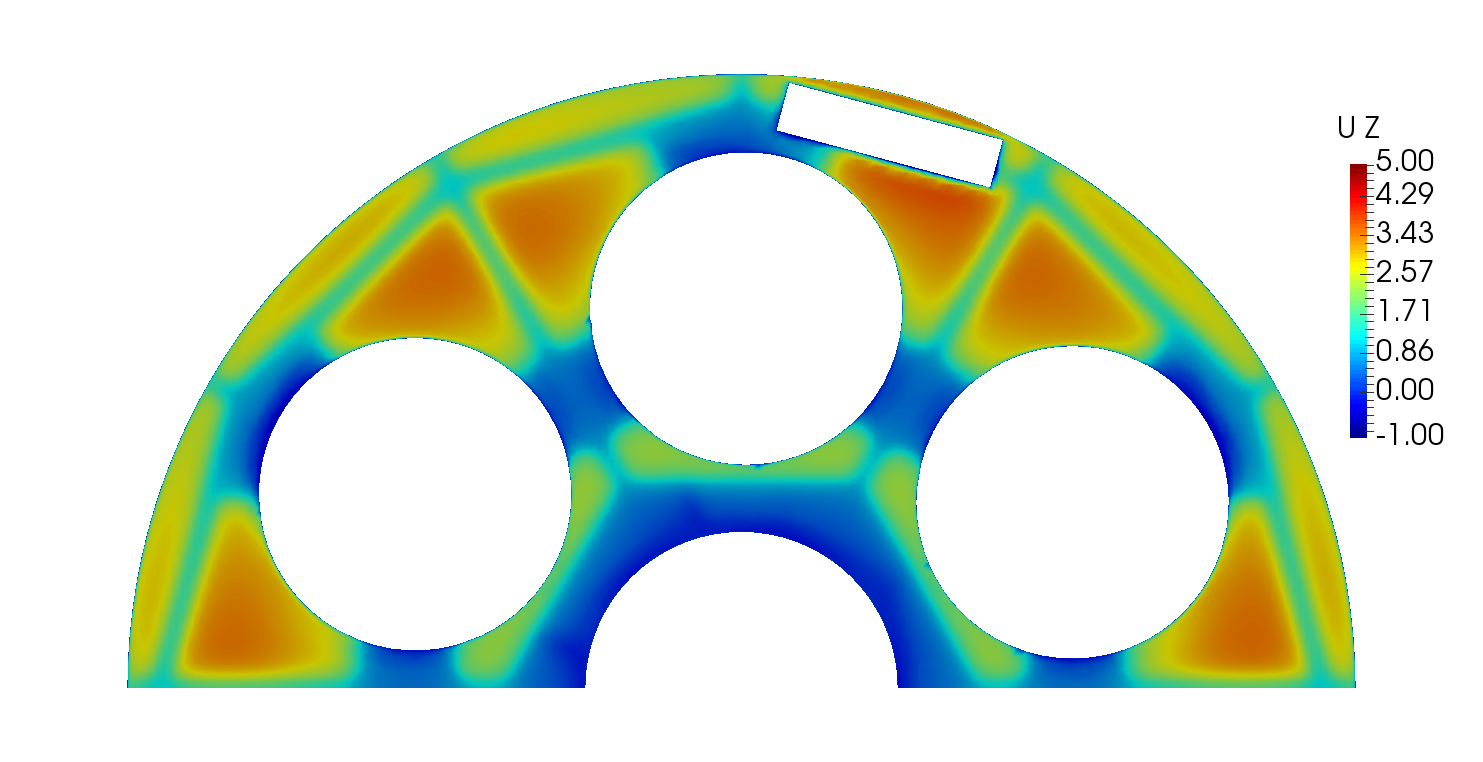
\includegraphics[width=0.45\textwidth]{figsATUCHA/vel/U_00075US.png}
             
            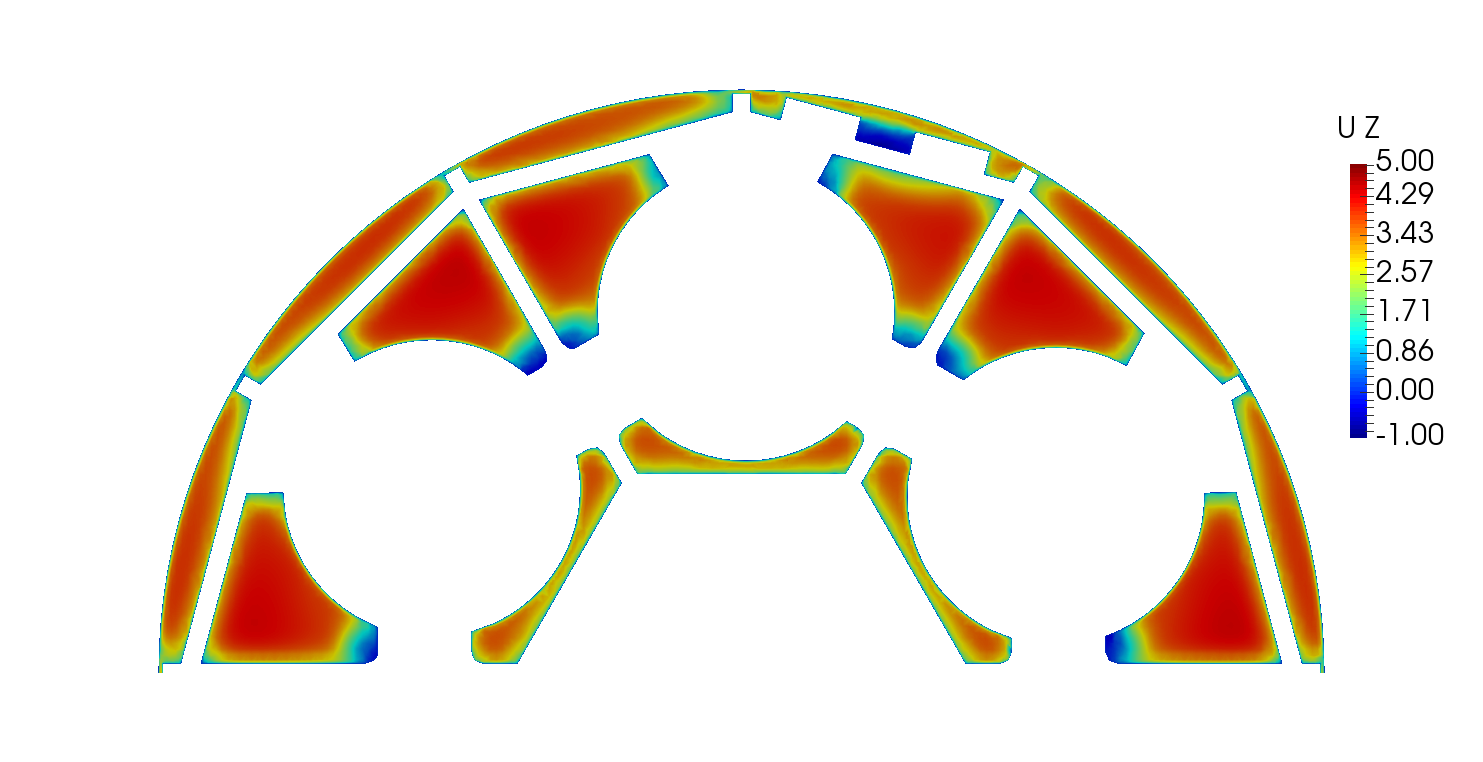
\includegraphics[width=0.45\textwidth]{figsATUCHA/vel/U_half.png}
             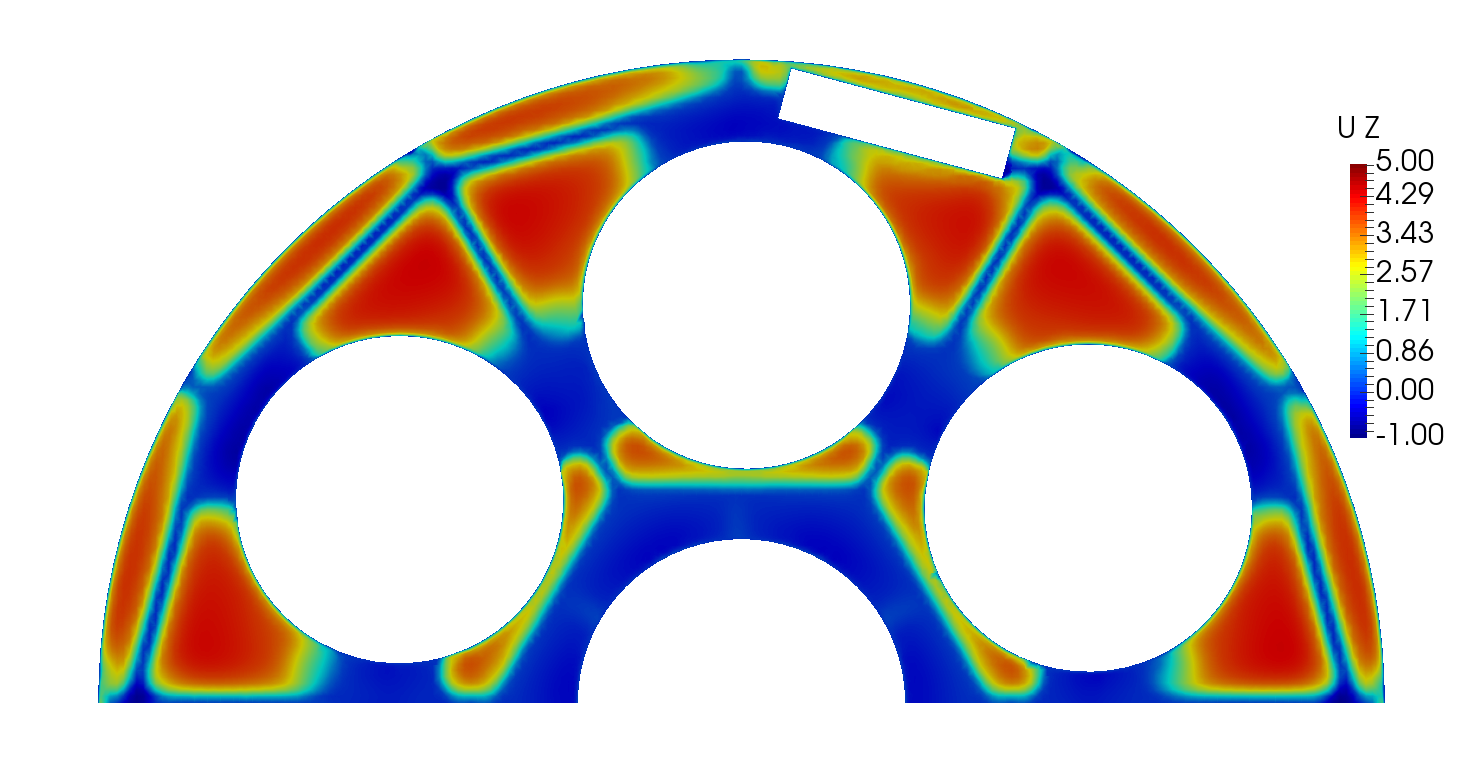
\includegraphics[width=0.45\textwidth]{figsATUCHA/vel/U_00075DS.png}
             
            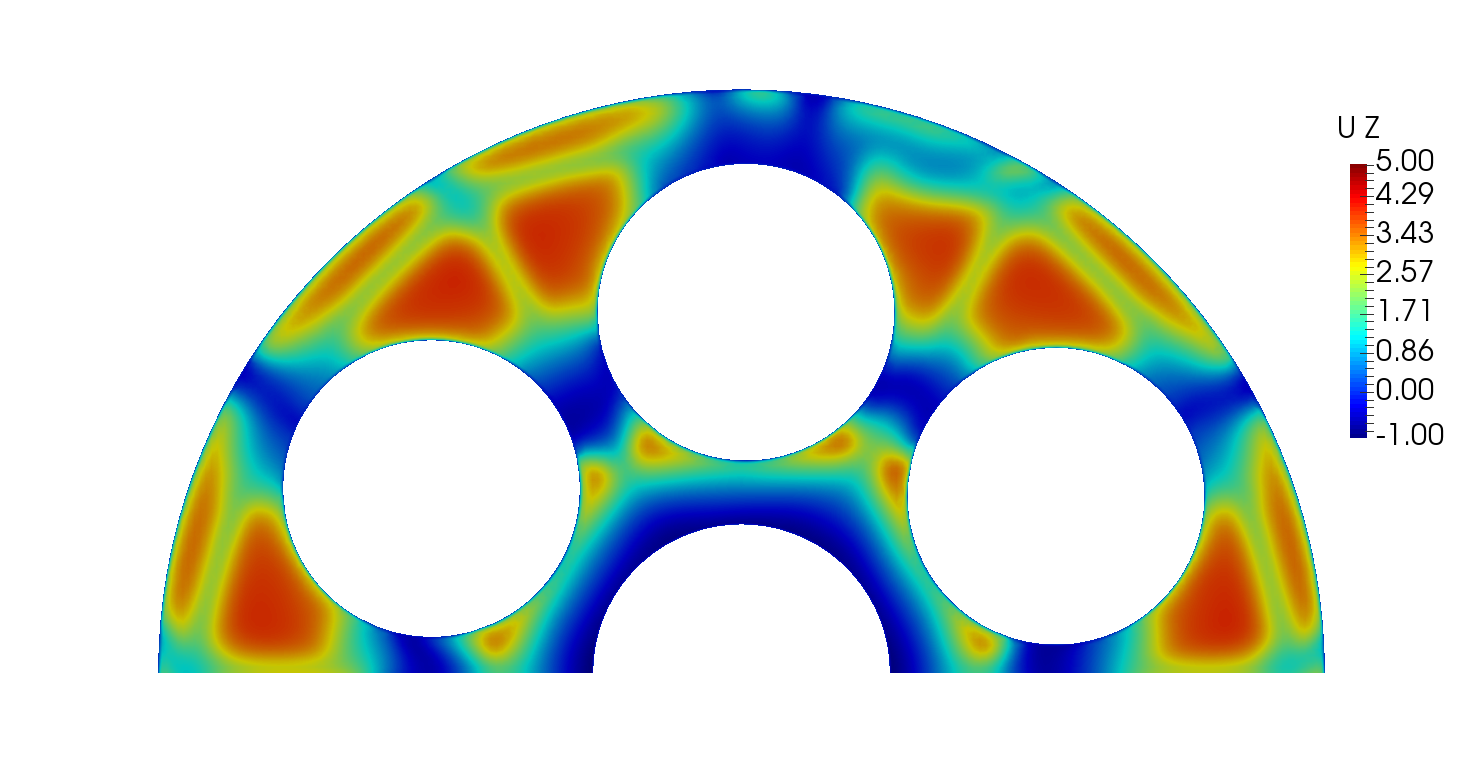
\includegraphics[width=0.45\textwidth]{figsATUCHA/vel/U_0015DS.png}
            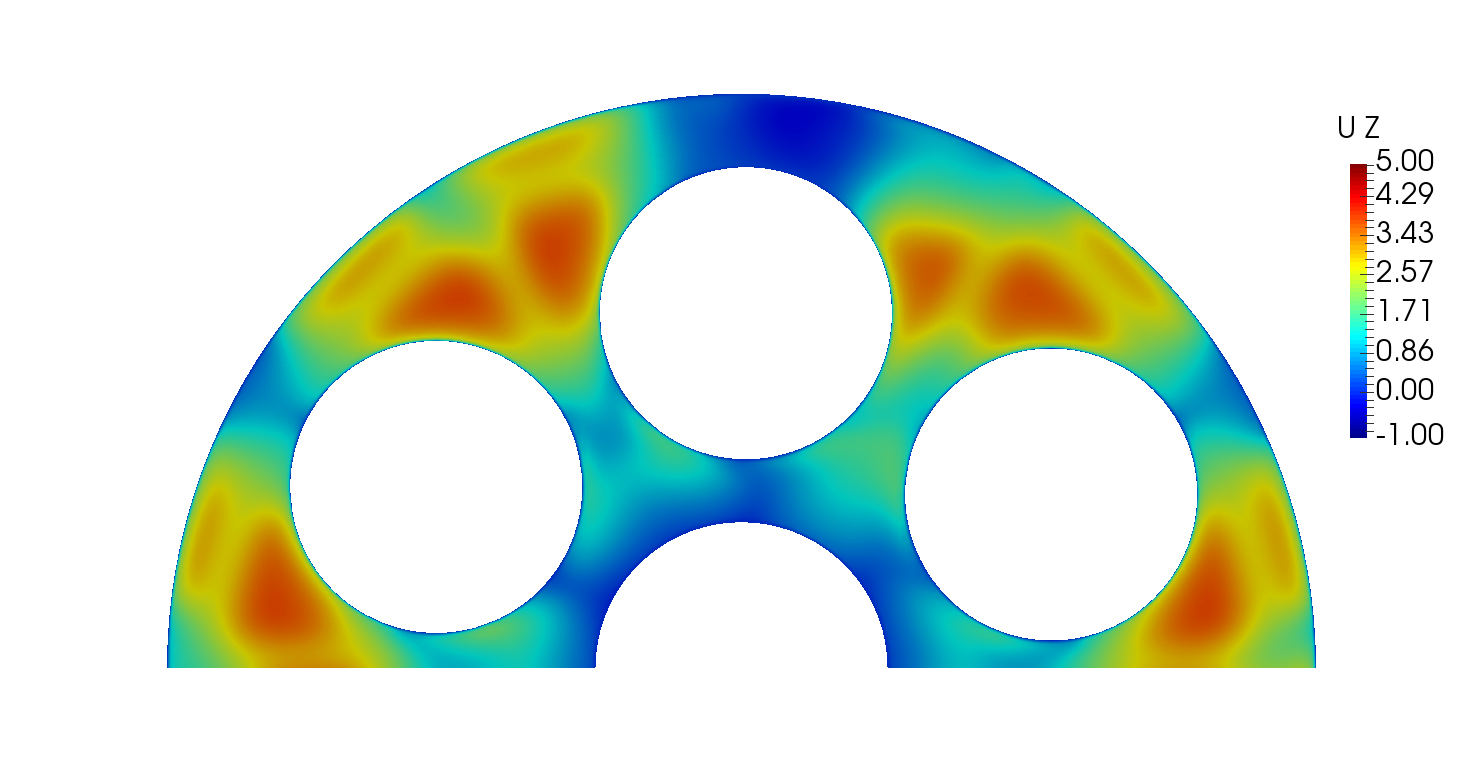
\includegraphics[width=0.45\textwidth]{figsATUCHA/vel/U_003DS.png} \vspace{-3mm}
        \caption{Distribución de la velocidad principal en secciones transversales: a) a 15mm US del separador, b) a 7.5mm US del separador, c) en la mitad del separador, d) a 7.5mm DS del separador, e) a 15mm DS del separador y f) a 30mm DS del separador.}
    \end{figure}
 }
% ==========================================================================================================
\subsection{EC CAREM}
\frame{
  \frametitle{Elemento combustible símil CAREM}
}

\section{Conclusiones}
\frame{
  \frametitle{Conclusiones}

  \begin{itemize}
    \item Se llevaron a cabo simulaciones RANS en OpenFOAM.
    \item Las geometrías se mallaron con la herramienta SnappyHexMesh de OpenFOAM.
    \item Se realizó un análisis previo de varios modelos de turbulencia en un canal simple.
    \item Se calculó la pérdida de carga en un EC símil CNAII de 7 vainas y se comparó con mediciones experimentales. Se obtuvieron diferencias del 30\%
    \item Se realizó el cálculo de un EC símil CAREM de 16 vainas.
   \end{itemize}
}

%% \frame[plain]{
%%   \begin{textblock}{15}(4.5,1.25)
%%     \normalsize{¡Gracias por su atención!}
%%   \end{textblock}
%%   \begin{textblock}{15}(2.25,5)
%%     \normalsize{ XXIII Congreso sobre Métodos Numéricos y sus Aplicaciones}
%%   \end{textblock}
%%   \begin{textblock}{5}(0,4.25)
%%     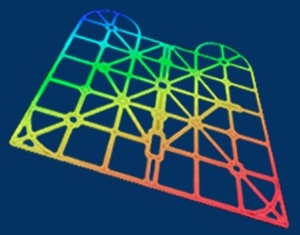
\includegraphics[width=1.5cm]{figuras/ENIEF2017.png}
%%   \end{textblock}
  
%%   %% \begin{textblock}{5}(12,-4)
%%   %%   
\includegraphics[width=1.25cm]{figuras/CNEA.jpg}
%%   %% \end{textblock}
%% }


\end{document}

